\section{Windows}
\subsection{Storia}
Negli anni '80 IBM stava sviluppando un nuovo personal computer, per il quale volevano utilizzare il sistema operativo CP/M di Digital Reserch.

Tuttavia il presidente non volle incontrare IBM, quindi essi andarono da Microsoft che sviluppò in breve tempo il sistema MS-DOS.

\spacer
Alla fine degli anni '80 MS-DOS acquisisce un'interfaccia utente e prende il nome di Windows.

\spacer
Nel 1993 Windows NT (New Technology) viene rilasciato, una completa riscrittura del sistema in quanto MS-DOS non era adatto ai computer del tempo.

\spacer
Nel 2006 Windows Vista porta una riprogettazione grafica del sistema.

\spacer
Con Windows 8 Microsoft prova ad avvicinarsi al mondo dei dispositivi mobile, con scarso successo, Windows 10 fornisce queste funzionalità, ma solamente agli utenti che ne necessitano invece che a tutti.

\subsection{Struttura del Sistema Operativo}

\begin{figure}[H]
    \centering
    \includegraphics[width=0.75\linewidth]{assets/Windows-structure.jpeg}
\end{figure}

Il primo strato sopra all'hardware è formato dall'hypervisor il quale gira sopra l'hardware e supporta l'esecuzione concorrente di più sistemi operativi.
Esso sfrutta le estensioni di virtualizzazione delle CPU per ripartire le risorse di CPU, memoria, ecc\dots

\spacer
Al di sopra troviamo l'HAL (Hardware Abstraction Layer), esso realizza l'astrazione di dettagli hardware di basso livello, come l'accesso ai registri o il DMA.

\spacer
Salendo ancora si arriva al livello kernel di NTOS, esso si occupa di operazioni low level di scheduling e sincronizzazione dei processi. Il resto del kernel, ovver il livello executive di NTOS, costruisce su questo livello, permettendo una programmazione simile a quella a livello utente.

\spacer
Infine il livello executive di NTOS è largamente indipendente dall'architettura e supporta una gran quantità di funzionalità:
\begin{sitemize}
    \item \textbf{Gestore degli oggetti:} gestisce gli oggetti in modalità kernel come processi, thread, file, semafori, dispositivi, driver di I/O e timer
    \item \textbf{Gestore dell'I/O:} Fornisce la struttura per implementare i driver dei dispositivi e vari servizi del sistema, infatti i driver offrono anche estensibilità al sistema operativo.
    \item \textbf{Gestore dei processi}
    \item \textbf{Gestore della memoria}
    \item \textbf{Gestore della cache}
    \item \textbf{Security Reference Monitor:} Impone complessi meccanismi di sicurezza, evoluti dai requisiti del dipartimento della difesa degli Stati Uniti.
    \item \textbf{Gestore della configurazione:} Implementa il registro di sistema che contiene i dati della configurazione di sistema.
\end{sitemize}

\subsection{Processi}

In Windows oltre a processi e thread vengono introdotti anche i job, che raggruppano più processi e le fibre, contesti di esecuzione schedulati in modo cooperativo.

\begin{figure}[H]
    \centering
    \includegraphics[width=0.75\linewidth]{assets/Windows-job.jpeg}
\end{figure}

Al contrario di unix la procedura di creazione di un thread non è così leggera come una chiamata a fork(), questo ha dei vantaggi, ma anche un aumento del tempo di esecuzione.

Per questo motivo possono essere usate delle thread pool, un gruppo di thread attivi a cui possono essere fornite delle istruzioni.

\subsubsection{Scheduler}
Windows utilizza delle classi di priorità sia sui processi che sui thread, ottenendo poi le vere priorità da una tabella.

I processi possono avere come priorità: real-time, alta, sopra al normale, normale, sotto al normale e inattivo.

I thread possono avere come priorità: time critical, altissima, sopra il normale, normale, sotto il normale, bassissima e inattivo.

\begin{figure}[H]
    \centering
    \includegraphics[width=0.75\linewidth]{assets/Windows-priority.jpeg}
\end{figure}

Il sistema mantiene poi 32 liste di thread e quando deve selezionare un processo prende il primo processo che trova scendendo le liste.

Dopo che il processo ha eseguito il suo quanto di tempo esso viene rimesso in coda alla stessa lista.

\spacer
Per migliorare la scalabilità dell'algoritmo più set di 32 liste possono esistere, alcune specifiche ad un singolo processore, altre comuni ad un set di processori.

\subsubsection{Emulazione x86}
Fino a Windows 7 per eseguire applicazioni a 32 bit su sistemi a 64 si utilizzava una macchina virtuale, tuttavia questo risulta inefficiente e difficile da nascondere all'utente.

L'approccio moderno è quello di utilizzare WoW64, uno strumento che traduce le chiamate a sistema delle applicazioni a 32 bit in chiamate a sistema per x64.

\subsubsection{Emulazione x64}
Su Windows 11 viene aggiunto il supporto per l'emulazione di applicazioni x64 su sistemi arm64.

I binari di sistema intesi per il caricamento di applicazioni x64 sono in un formato ARM64EC (Emulation Compatible), ovvero codice macchina arm64 compilato con comportamento e tipi per x64.

Il resto dei binari di sistema sono compilati in ARM64X, e contengono sia codice arm64 che codice compatibile con x64, in base al processo richiedente viene caricata la versione corretta.

\subsection{Gestione della memoria}
Windows utilizza 48 bit per l'indicizzazione della memoria, fornendo 258 TB di memoria ai processi, 128 per la modalità utente e 128 per la modalità kernel.

Utilizza una paginazione pura a 4 livelli con pagine di 4KB, 2MB o 1GB.

\spacer
Le pagine virtuali sono dette \textbf{non valide} finché non sono mappate ad un oggetto, vegnono poi dette \textbf{committed} quando una pagina fisica può venir allocata su richiesta.
Infine le pagine virutali possono essere \textbf{riserved}, per indicare che sono libere, ma assegnate ad un processo.

\spacer
Windows ha diverse funzionalità di prefetching:
\begin{sitemize}
    \item Quando avviene un page fault Windows carica sempre 64KB di memoria, includendo pagine vicine al page fault.
    \item Quando viene avviata un'applicazione Windows salva le pagine che vengono subito utilizzate e le carica in memoria ai riavvii successivi.
    \item \textbf{Superfetch} ovvero il fetching di pagine spesso utilizzate quando il sistema è in idle.
\end{sitemize}

\subsection{Gestione dell'I/O}
Windows include il supporto per il plug-and-play che permette al sistema di rilevare e configurare automaticamente i nuovi dispositivi hardware.

I driver dei dispositivi devono essere conformi con il Windows Drier Model e spesso vegnono eseguiti in modalità utente, così da limitare i possibili danni di un errore.

\subsection{File System}
Windows supporta diversi file system, i più importanti dei quali sono FAT-16, FAT-32, NTFS (NT File System) e ReFS (Resilient File System).

ReFS è il file system più nuovo, prende il nome di Resilient File System perché uno dei suoi obiettivi progettuali è ripararsi da solo: può verificarsi e ripararsi automaticamente senza downtime.
Ciò è possibile mantenendo metadati di integrità per le strutture dati su disco, oltre che per i dati utente.

\subsubsection{NTFS}
NTFS, come ext4 è un file system Journaled, sviluppato assieme a Windows NT ed è di default da quel momento.

\spacer
I nomi dei file NTFS sono unicode con un limite di 255 caratteri, quindi tutti possono utilizzare la propria lingua nello scrivere il nome dei file.
\spacer
Ciascun volume NTFS è organizzato come una sequenza lineare di blocchi spesso di 4 KB come compromesso tra blocchi grandi (per trasferimenti efficaci) e blocchi piccoli (per la ridotta frammentazione interna).
\spacer
La struttura dati principale in ciascun volume è la MFT (Master File Table), una sequenza lineare di record di file e directory.
Ciascun elemento della tabella contiene gli attributi del file, come il suo nome e i timbri temporali, e la lista degli indirizzi del disco dove sono posizionati i suoi blocchi. Se un file è estremamente grande, qualche volta è necessario usare due o più record della MFT per contenere la lista di tutti i blocchi, e in tal caso il primo record della MFT, chiamato record base, punta agli altri record della MFT.

\spacer
Vediamo una tipica MFT per un file di 9 blocchi.
\begin{figure}[H]
    \centering
    \includegraphics[width=0.75\linewidth]{assets/Windows-MFT.jpeg}
\end{figure}

NTFS supporta anche la compressione trasparente all'utente, essa funziona nel seguente modo:
Il file viene diviso in sezioni di 16 blocchi, su ogniuna si prova ad applicare un algoritmo di compressione, se il risultato è di 15 blocchi o meno quella sezione del file viene compressa e scritta.

\begin{figure}[H]
    \centering
    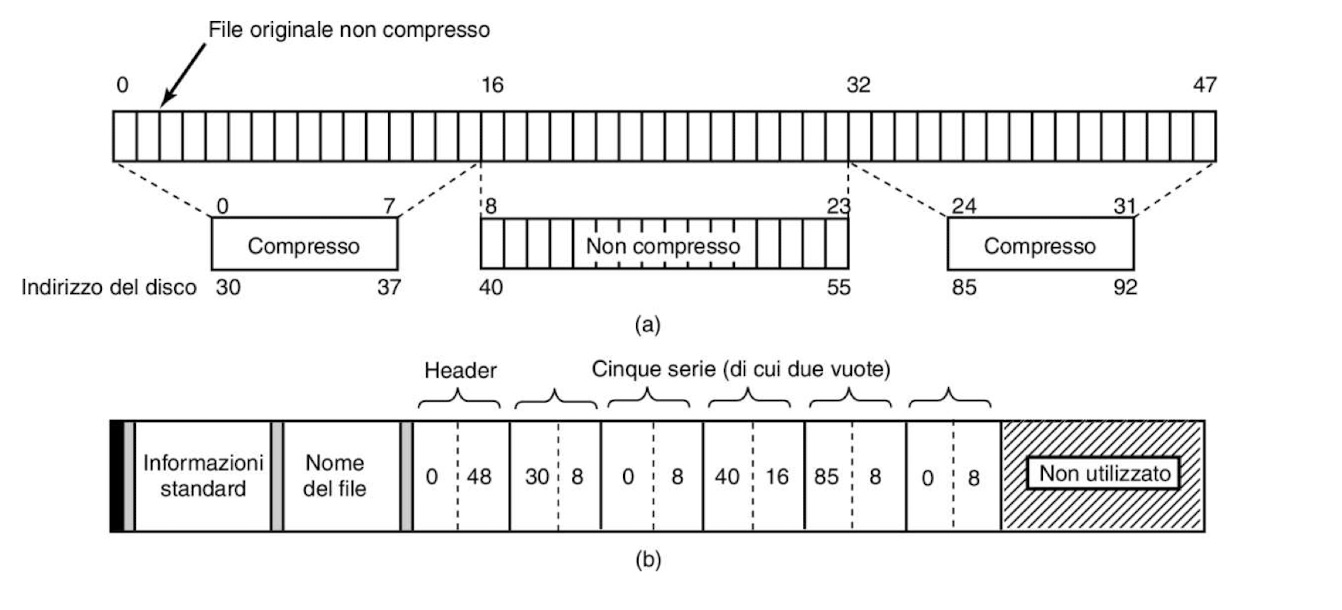
\includegraphics[width=0.75\linewidth]{assets/windows-MFT-compression.jpeg}
\end{figure}

Windows infine fornisce anche Bitlocker, uno strumento di cifratura del disco, questo è particolarmente utile per i laptop che sono più semplici da smarrire o rubare.